\section{Calorimeter Noise simulation}
\label{sc:CaloNoise}

Fluctuations in the calorimeter electronics noise can be a source of a small amount of missing energy. Therefore, the first step
in making comparisons between Monte Carlo simulation and data is to look at the detector noise and its simulation. For this purpose
events from the following two samples were used:

\begin{itemize}
  \item Noise-only sample: \newline
This sample was produced in CMSSW\_3\_3\_6\_path3 by generating single electron neutrinos with the rest of the configuration identical to the one used to
produce /MinBias/Summer09-STARTUP3X\_V8P\_900GeV-v1/GEN-SIM-RECO dataset. No special event selection was applied.

  \item /ZeroBias/BeamCommissioning09-Jan23ReReco-v1/RECO: \newline
ZeroBias dataset is formed from the OR between the following BPTX triggers: BPTX\_PlusOnly, BPTX\_MinusOnly, BPTX\_Plus
OR BPTX\_Minus, and BPTX\_Plus AND BPTX\_Minus. Events selected from this dataset were required to pass the
veto on TT bit 0 (BPTX\_Plus AND BPTX\_Minus), i.e., bunch crossings corresponding to the beam-beam
collisions were excluded from the selection. Events selected in this way are almost completely noise-dominated. No event cleanup was applied.
\end{itemize}

Figure~\ref{fig:subdet_RecHitE} shows the comparison between RecHit energy distributions in noise-only and selected ZeroBias data for different
calorimeter sub-detectors. From plots in Figure~\ref{fig:subdet_RecHitE} it follows, with the exception of HF, that
the noise simulation reproduces reasonably well the bulk properties of the RecHit energy distributions. The reason for large discrepancy in HF lies 
in the fact that the zero-suppression threshold in HF is higher than in the other HCAL subdetectors and therefore more sensistive to the noise tails
which are not properly simulated. Figure~\ref{fig:subdet_CaloSumET} shows the comparison between $\sumet$ distributions in noise-only
and selected ZeroBias data in different calorimeter sub-detectors. Plots in Figure~\ref{fig:subdet_CaloSumET} reveal that the noise correlation
effects among neighbouring channels might not be properly modeled considering the level of agreement at the RecHit level, in particular in the
HCAL barrel (HB). The spikes in the $\sumet$ distributions in EB, EE, HB, and HE are due to the offline zero-suppression
thresholds applied to the ECAL and HCAL RecHits in the process of calotower formation. A relatively large discrepancy between HF noise in data and
Monte Carlo simulation in the end has a negligible effect on the MET-related quantities 
because of the high $\eta$ location of the HF cells. Part that has a non-negligible effect on the MET-related quantities are the PMT window hits
clearly visible in the HF plots in Figure~\ref{fig:subdet_CaloSumET} as entries outside the first bin. Since these
hits are correlated with the beam activity, they can also be caused by a single beam passing through the CMS detector and therefore can end up
in the selected ZeroBias events.

In order to understand if discrepancies between data and Monte Carlo simulation are coming from a specific region of the detector, it is useful to
look at the mean and RMS of the $\sumet$ distributions in different $\eta$ slices of the calorimeter system. The $\sumet$ distributions in different
$\eta$ slices are obtained
by summing the transverse energy of calotowers with the same $\eta$ index ($i\eta$) and different $\phi$ indices ($i\phi$).
Figure~\ref{fig:SumET_MeanRMS_vs_ieta_ZB} shows the mean and RMS of such $\sumet$ distributions in different $i\eta$ rings. From the figure it is
immediately noticeable that the calotower $E_{\rm T}$ cut of $0.3$~GeV completely suppresses any noise contribution in the very forward region.
However, at the same it is also noticebale that the largest discrepancy exists in the most central region.


\begin{figure}[h!]
 \centering
 \begin{tabular}{ll}
  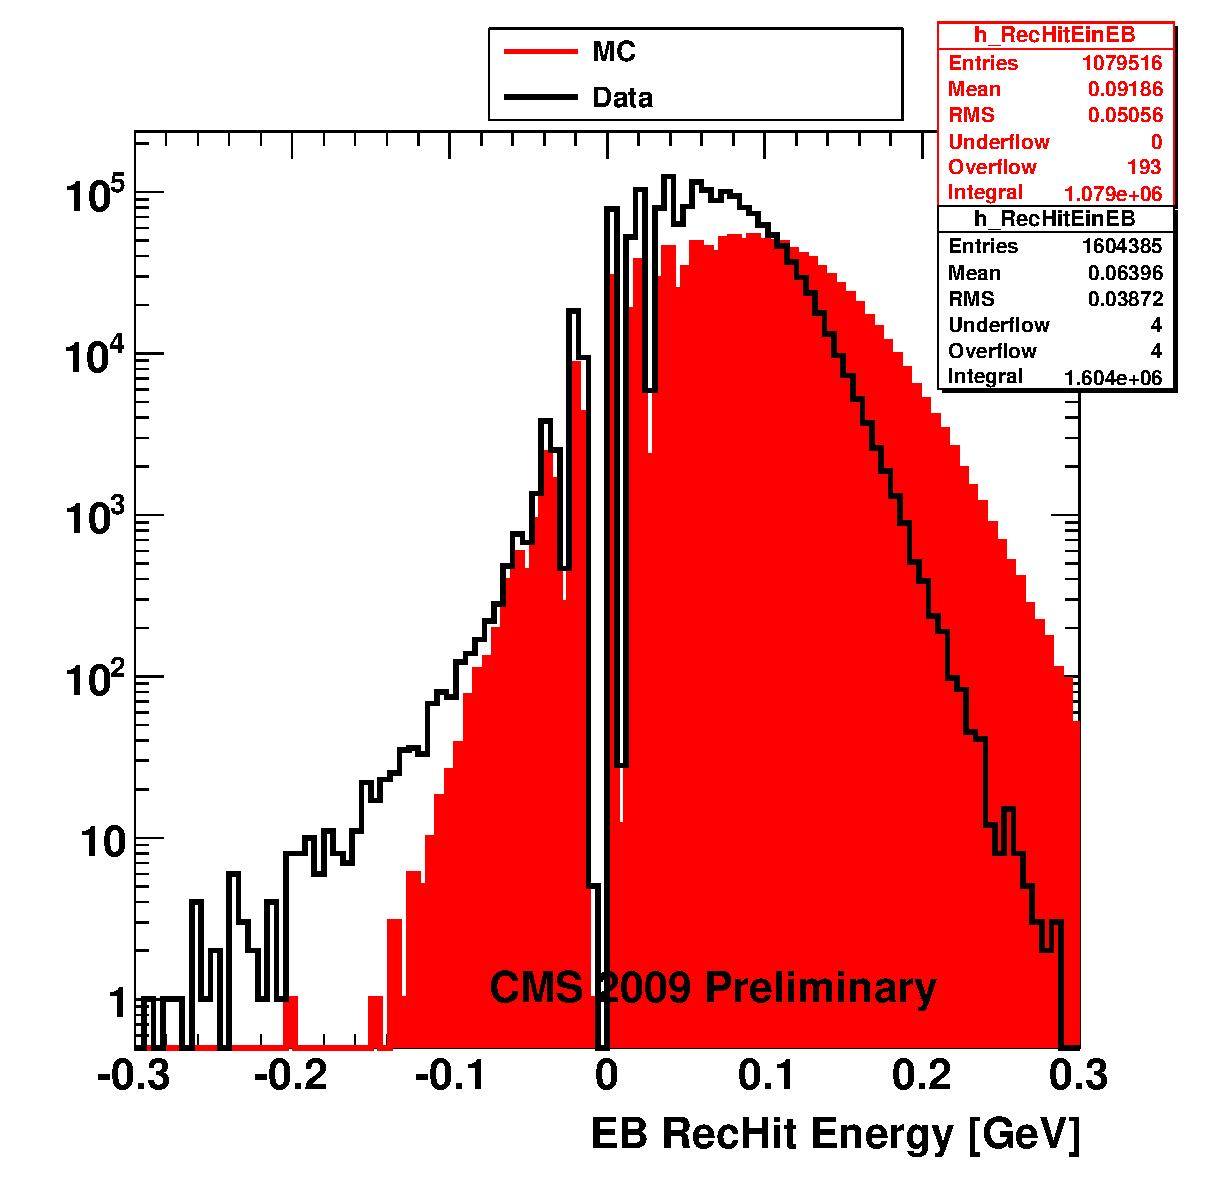
\includegraphics[width=0.33\textwidth]{plots_CaloNoise/h_RecHitEinEB.eps} &
  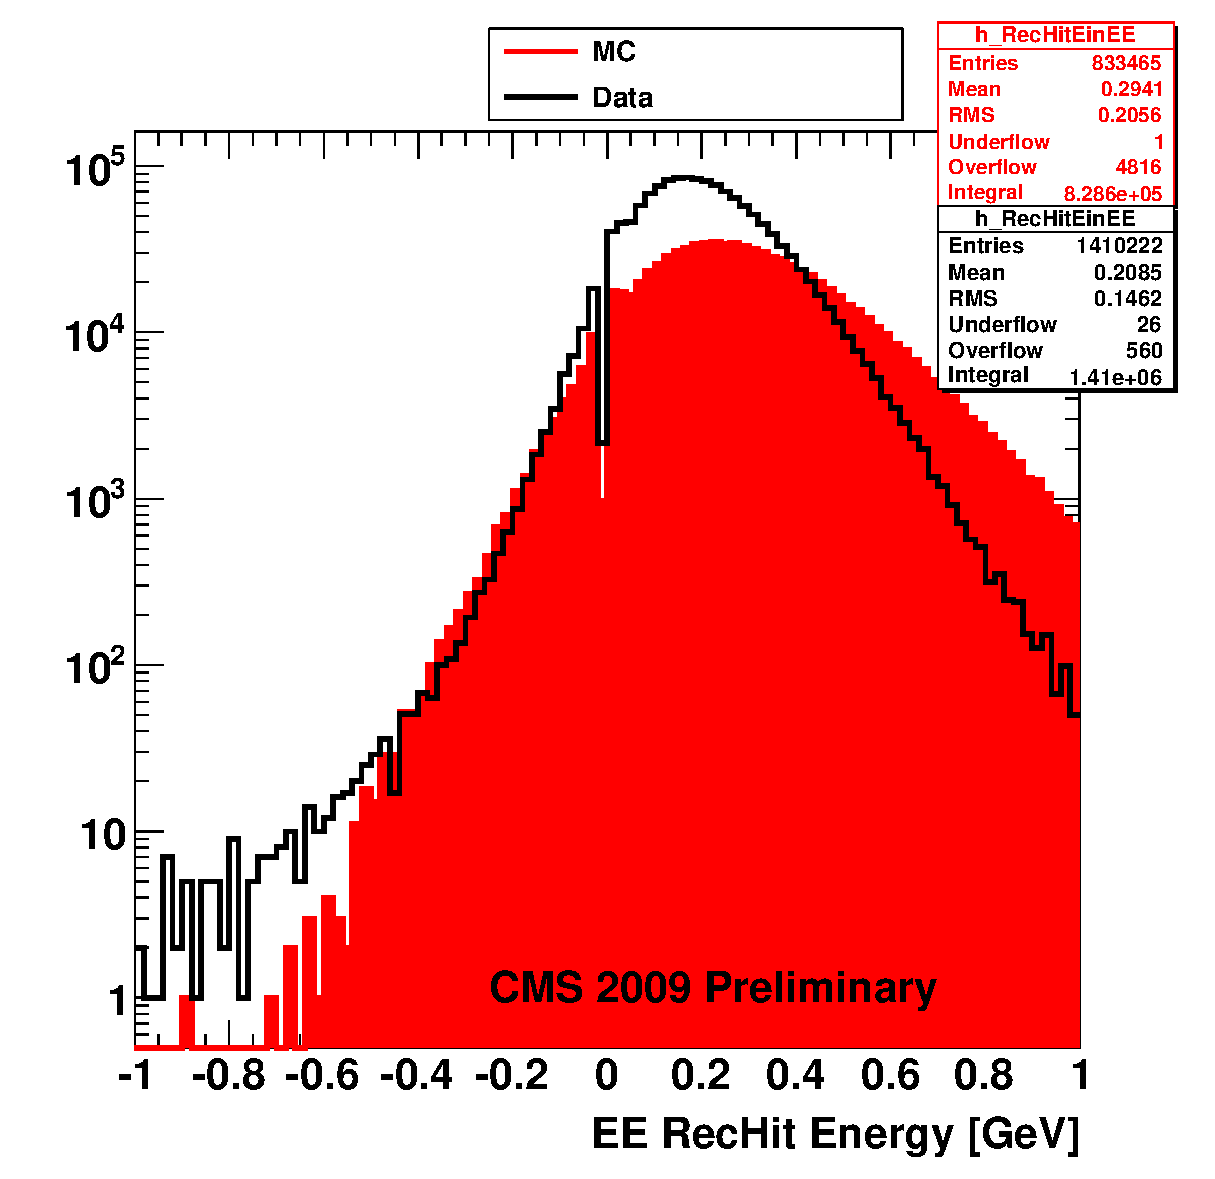
\includegraphics[width=0.33\textwidth]{plots_CaloNoise/h_RecHitEinEE.eps} \\
  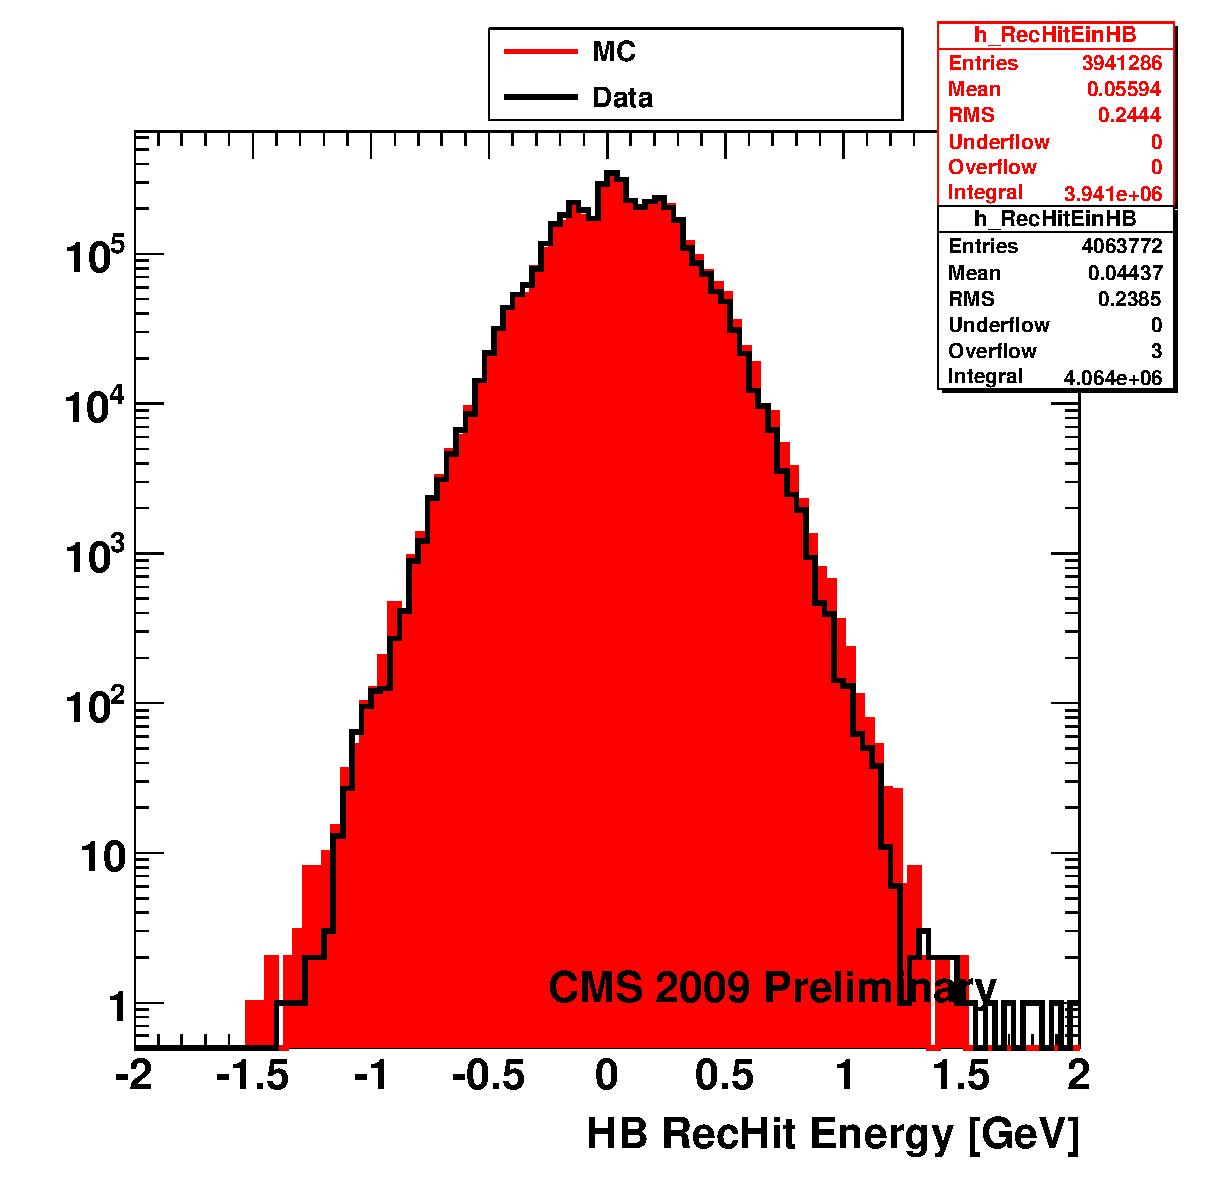
\includegraphics[width=0.33\textwidth]{plots_CaloNoise/h_RecHitEinHB.eps} &
  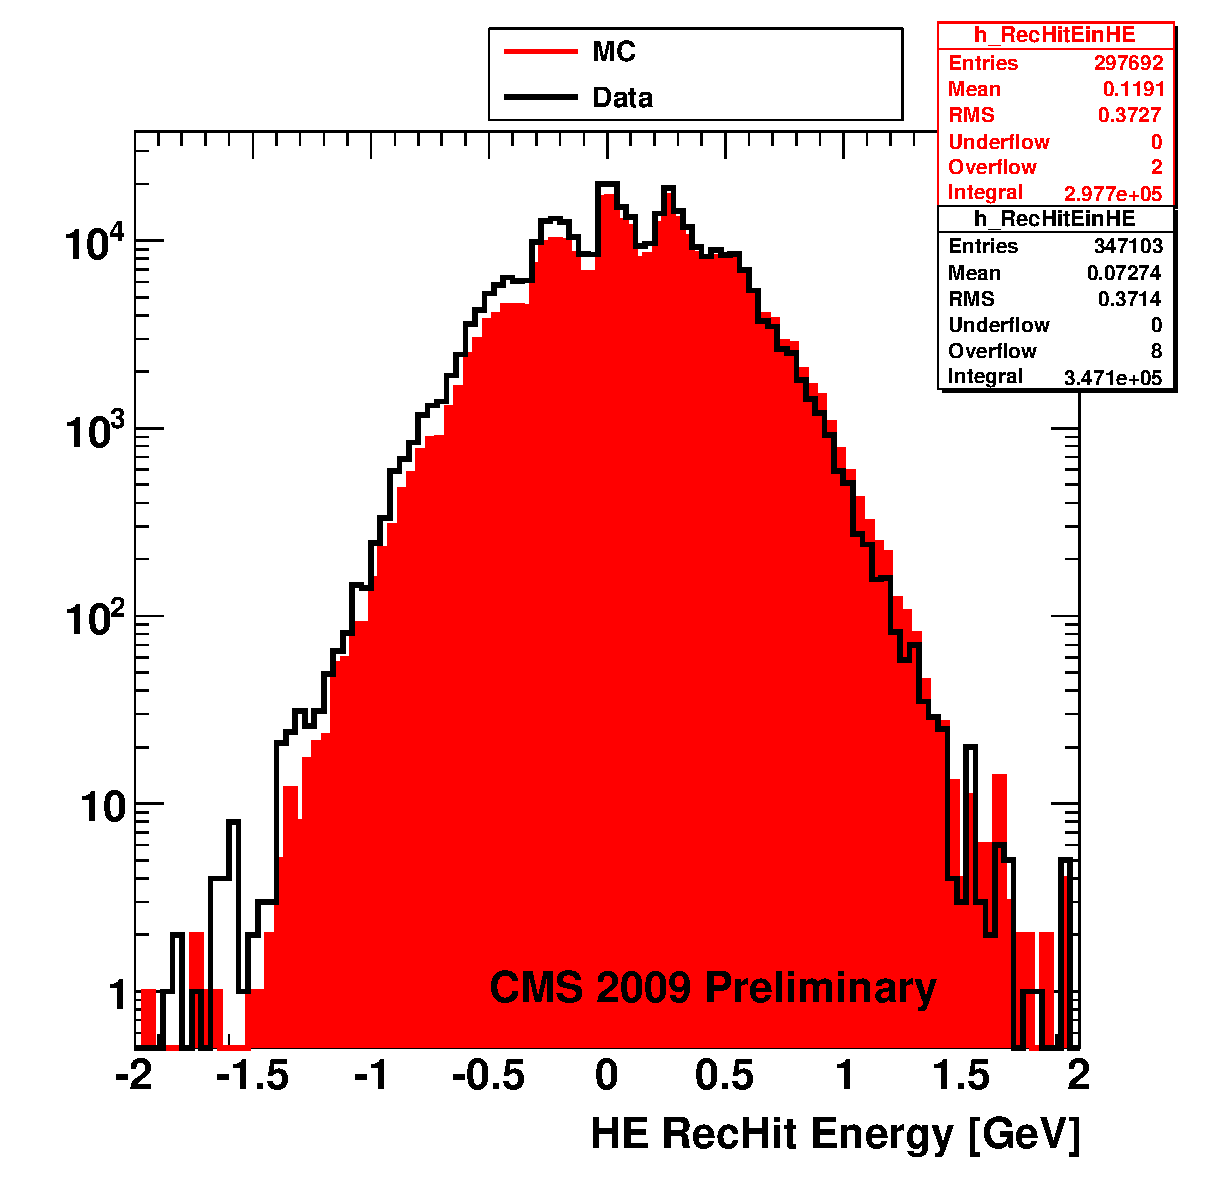
\includegraphics[width=0.33\textwidth]{plots_CaloNoise/h_RecHitEinHE.eps} \\
  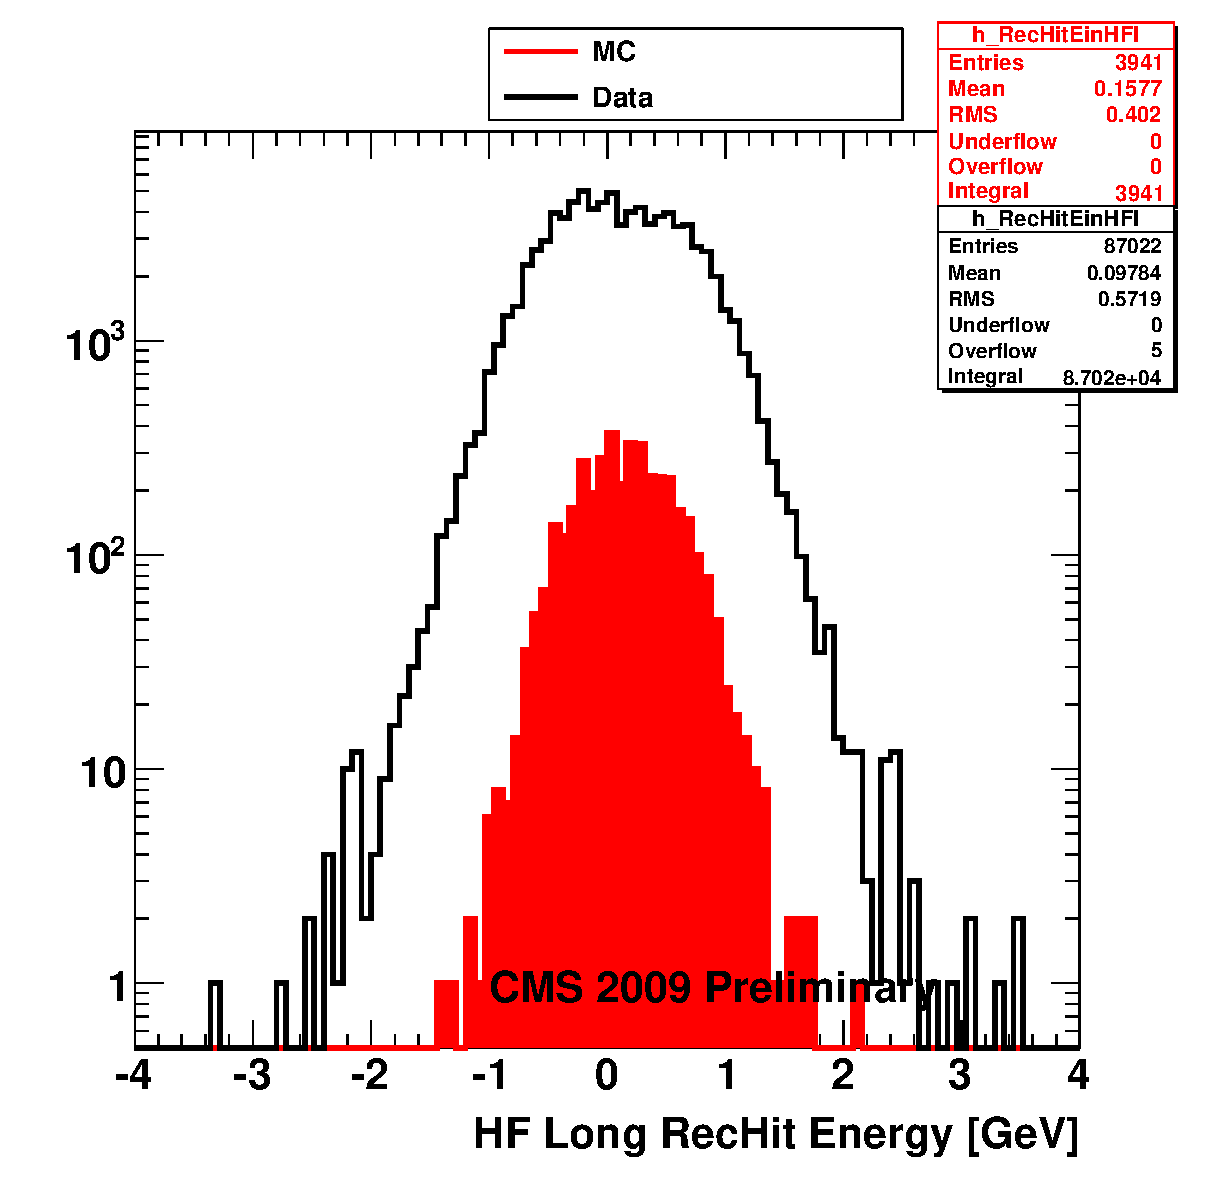
\includegraphics[width=0.33\textwidth]{plots_CaloNoise/h_RecHitEinHFl.eps} &
  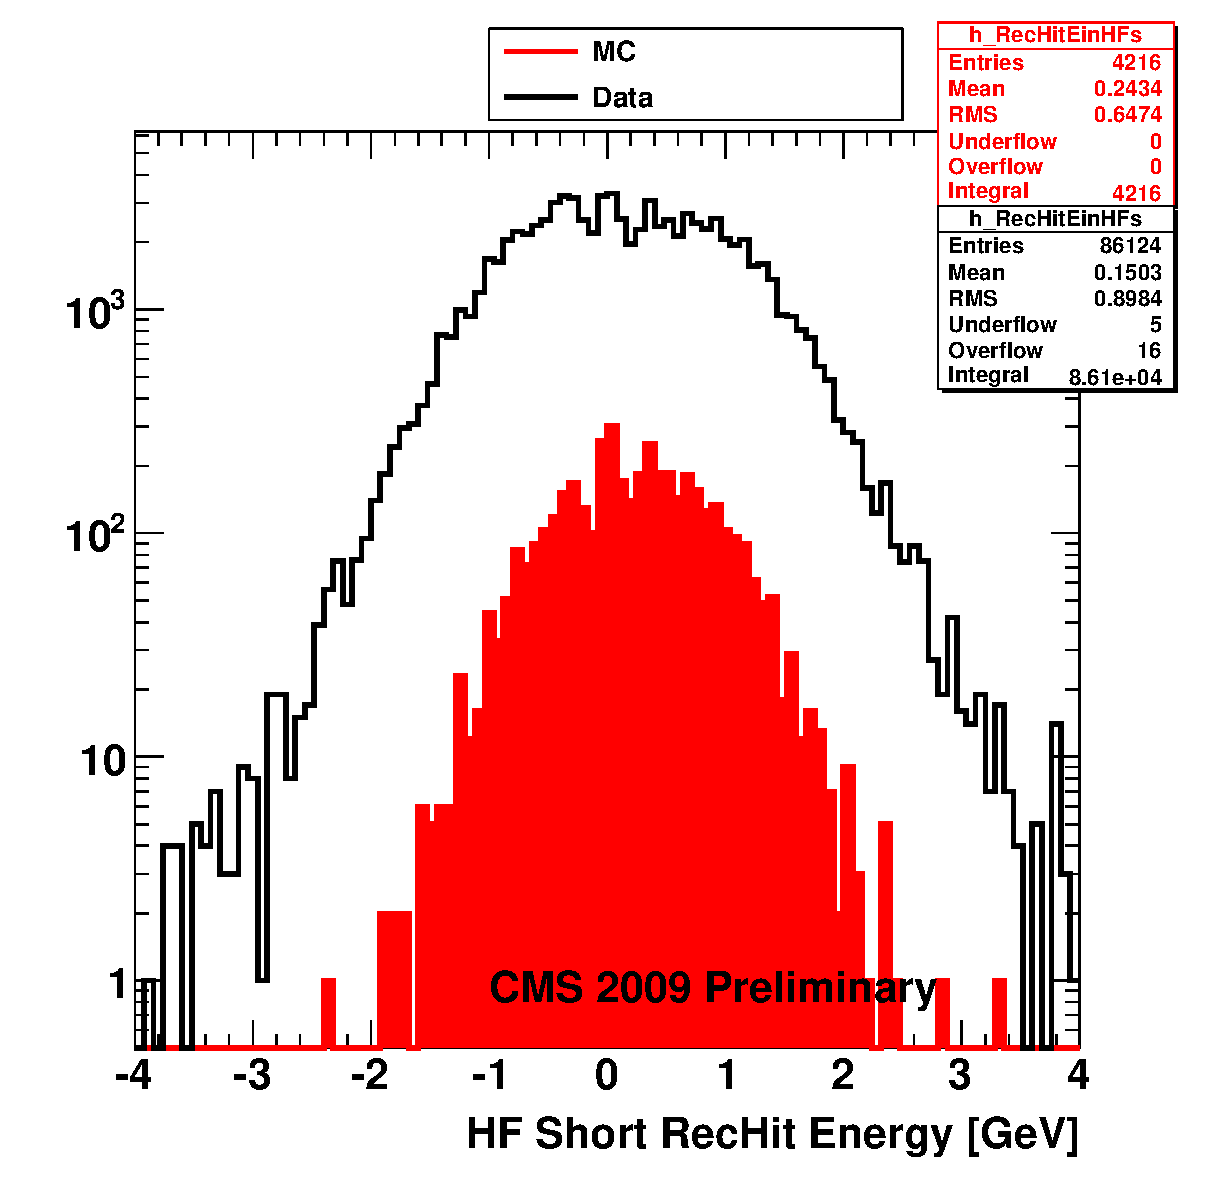
\includegraphics[width=0.33\textwidth]{plots_CaloNoise/h_RecHitEinHFs.eps} \\
 \end{tabular}
 \caption{\small RecHit energy distributions in noise-only (red-filled area) and selected ZeroBias data (black line) from
run 124022 for different calorimeter sub-detectors. The distributions shown are not normalized but correspond to the same number of events 
(5000 events).\label{fig:subdet_RecHitE}}
\end{figure}

\begin{figure}[h!]
 \centering
 \begin{tabular}{ll}
  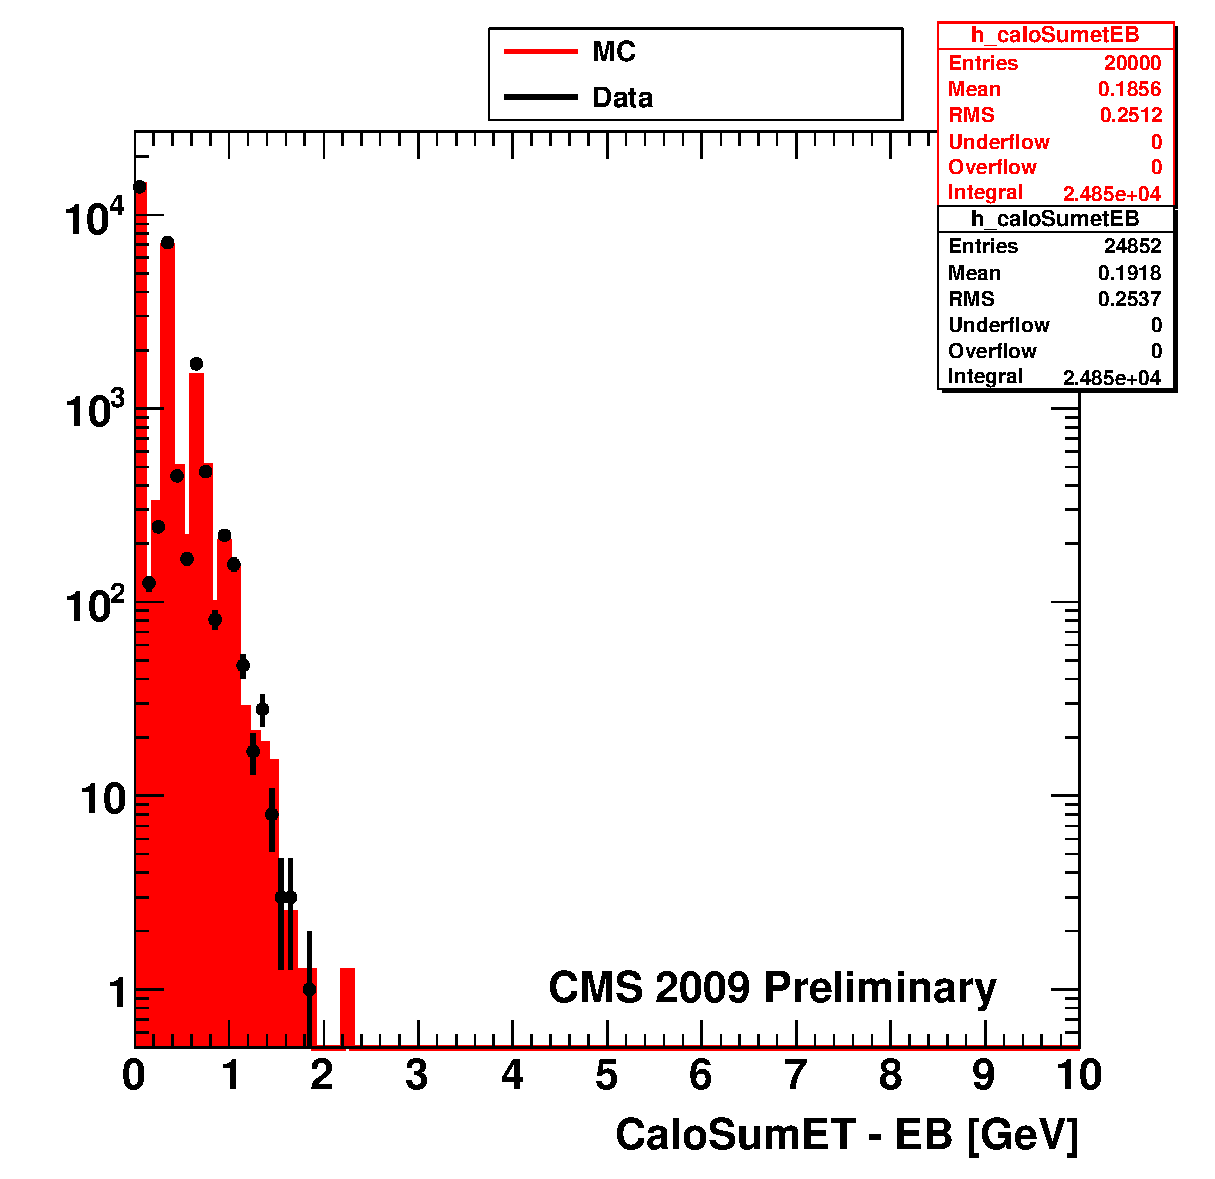
\includegraphics[width=0.33\textwidth]{plots_CaloNoise/h_caloSumetEB.eps} &
  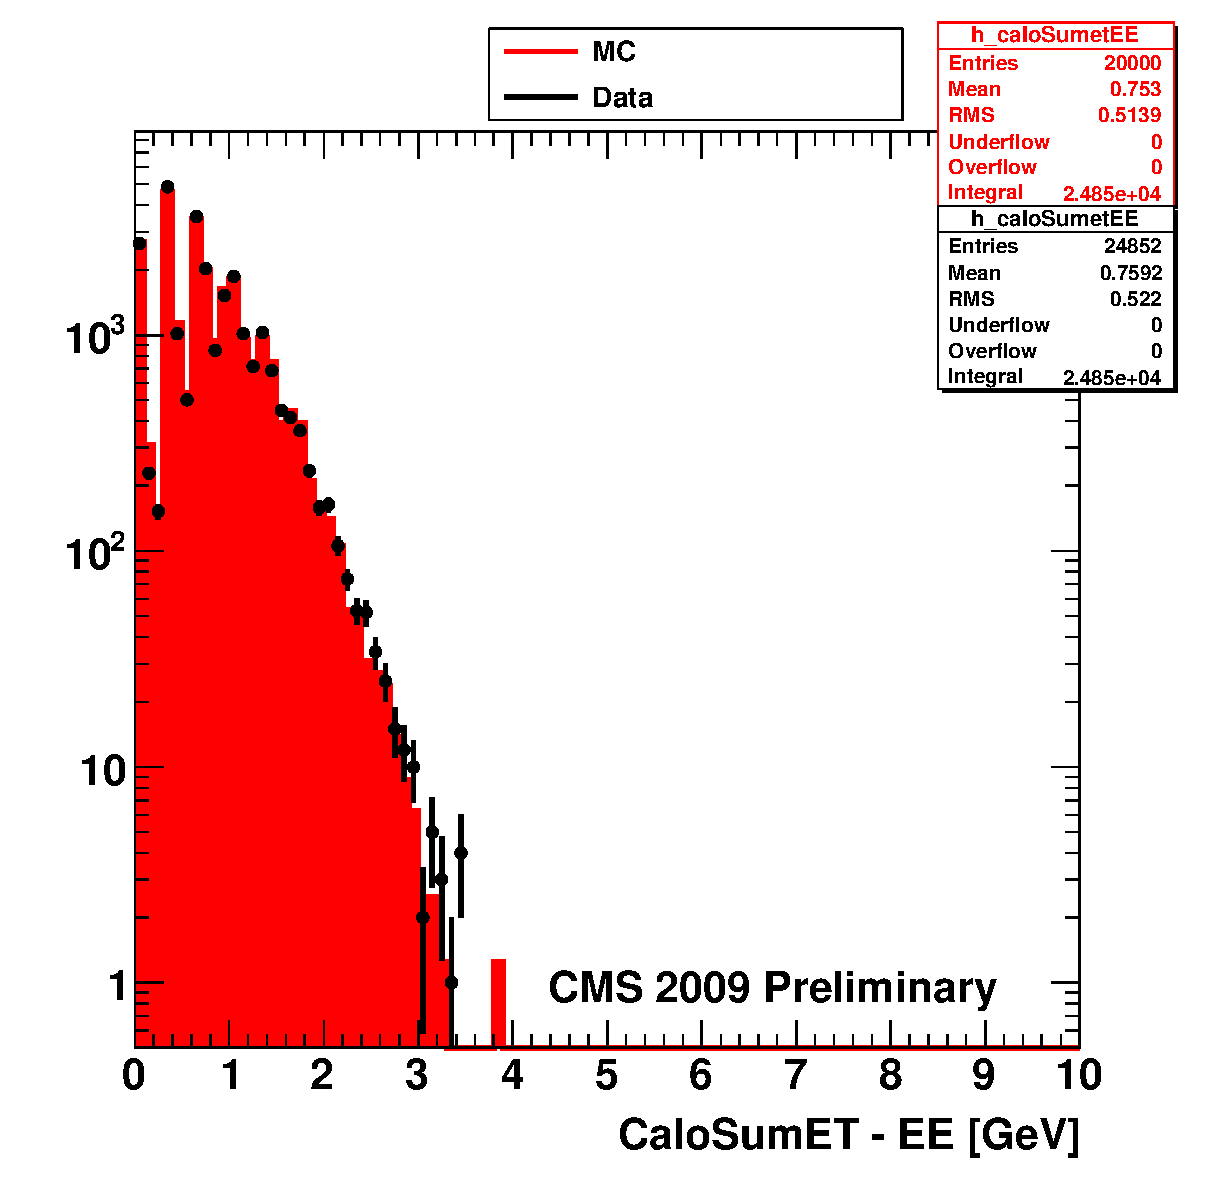
\includegraphics[width=0.33\textwidth]{plots_CaloNoise/h_caloSumetEE.eps} \\
  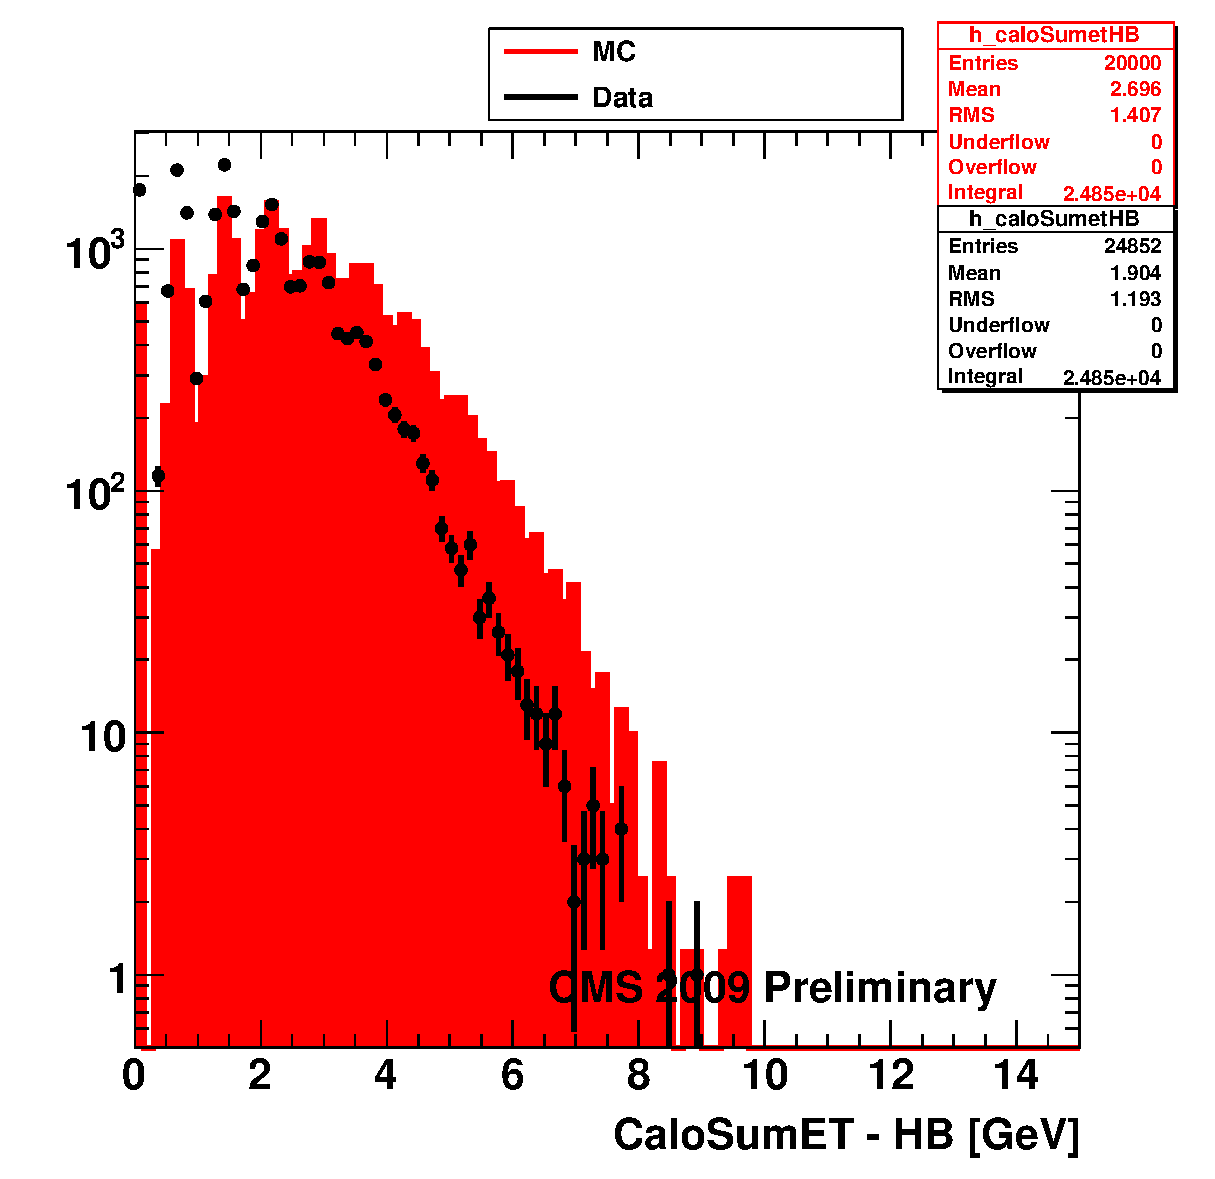
\includegraphics[width=0.33\textwidth]{plots_CaloNoise/h_caloSumetHB.eps} &
  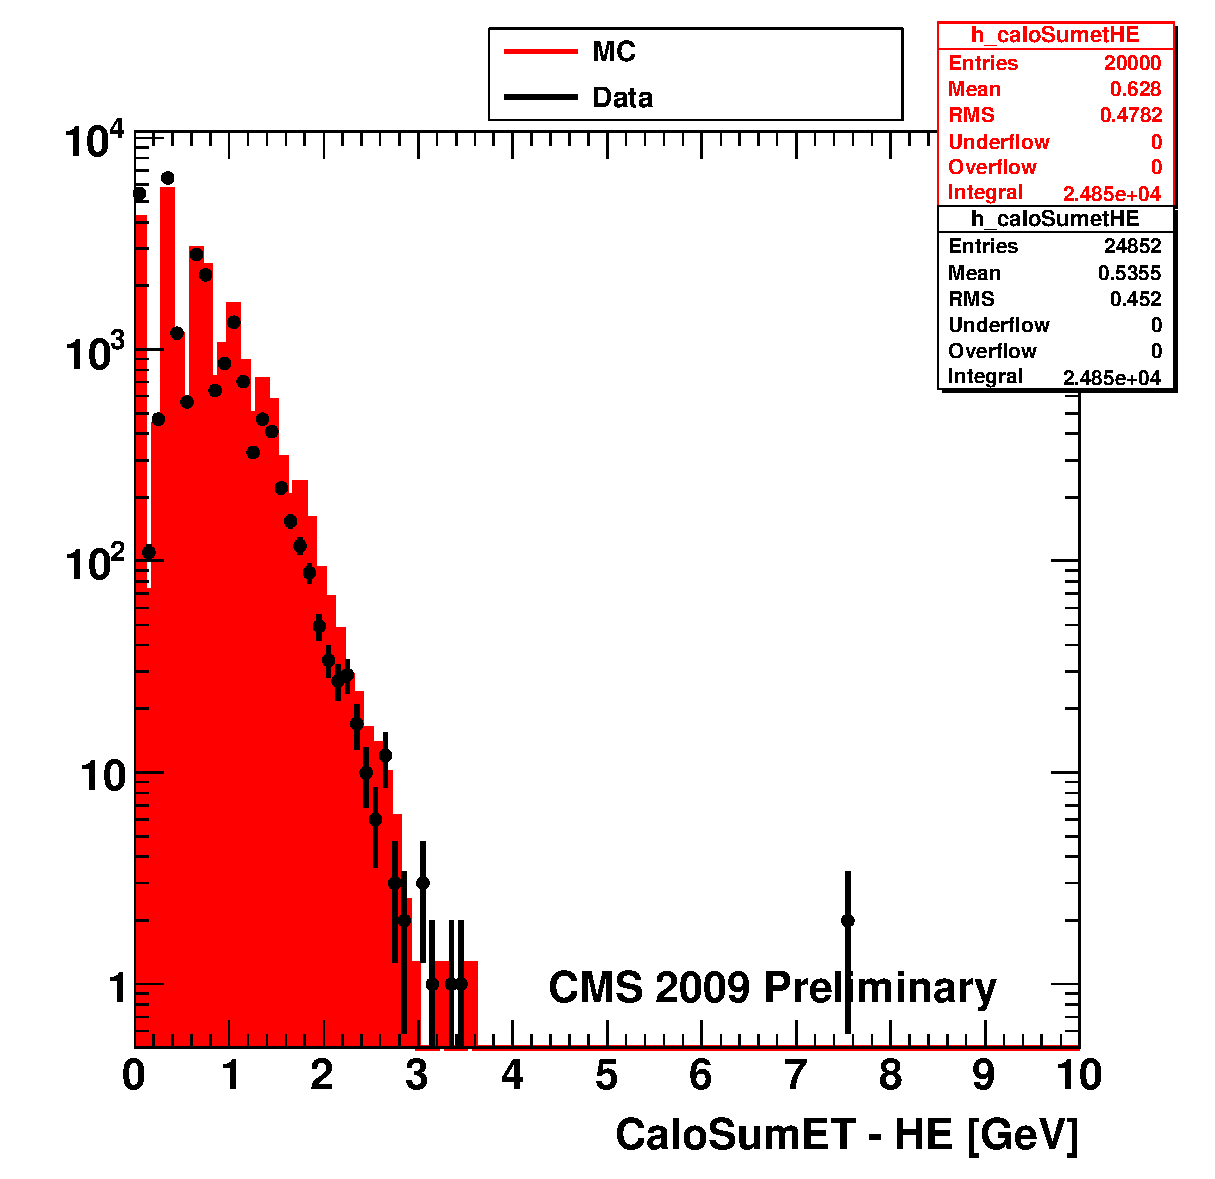
\includegraphics[width=0.33\textwidth]{plots_CaloNoise/h_caloSumetHE.eps} \\
  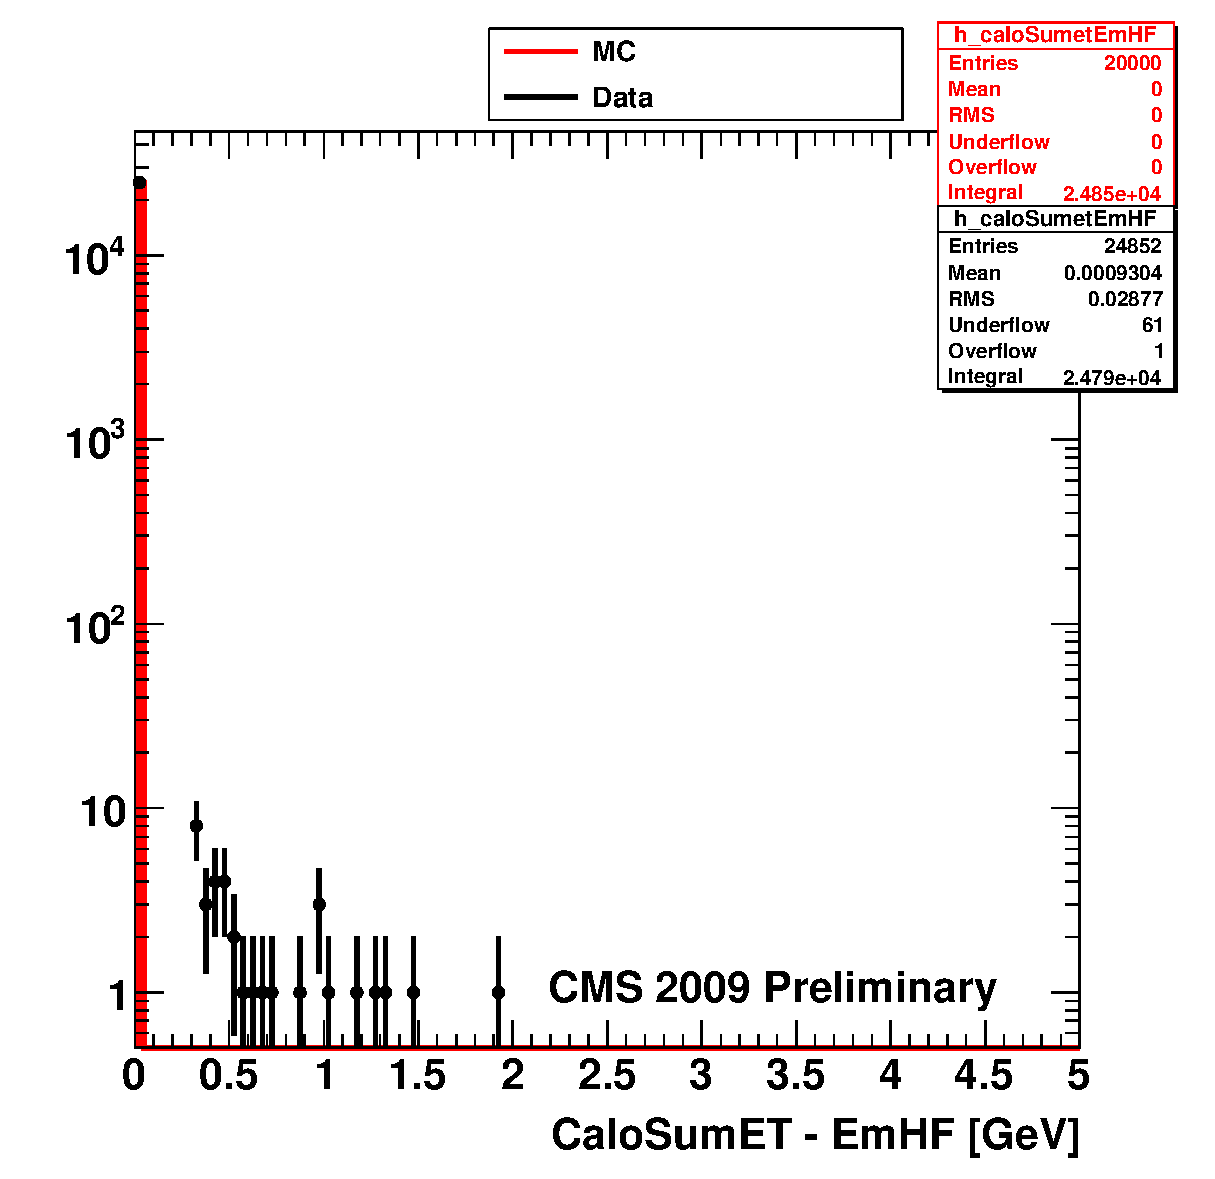
\includegraphics[width=0.33\textwidth]{plots_CaloNoise/h_caloSumetEmHF.eps} &
  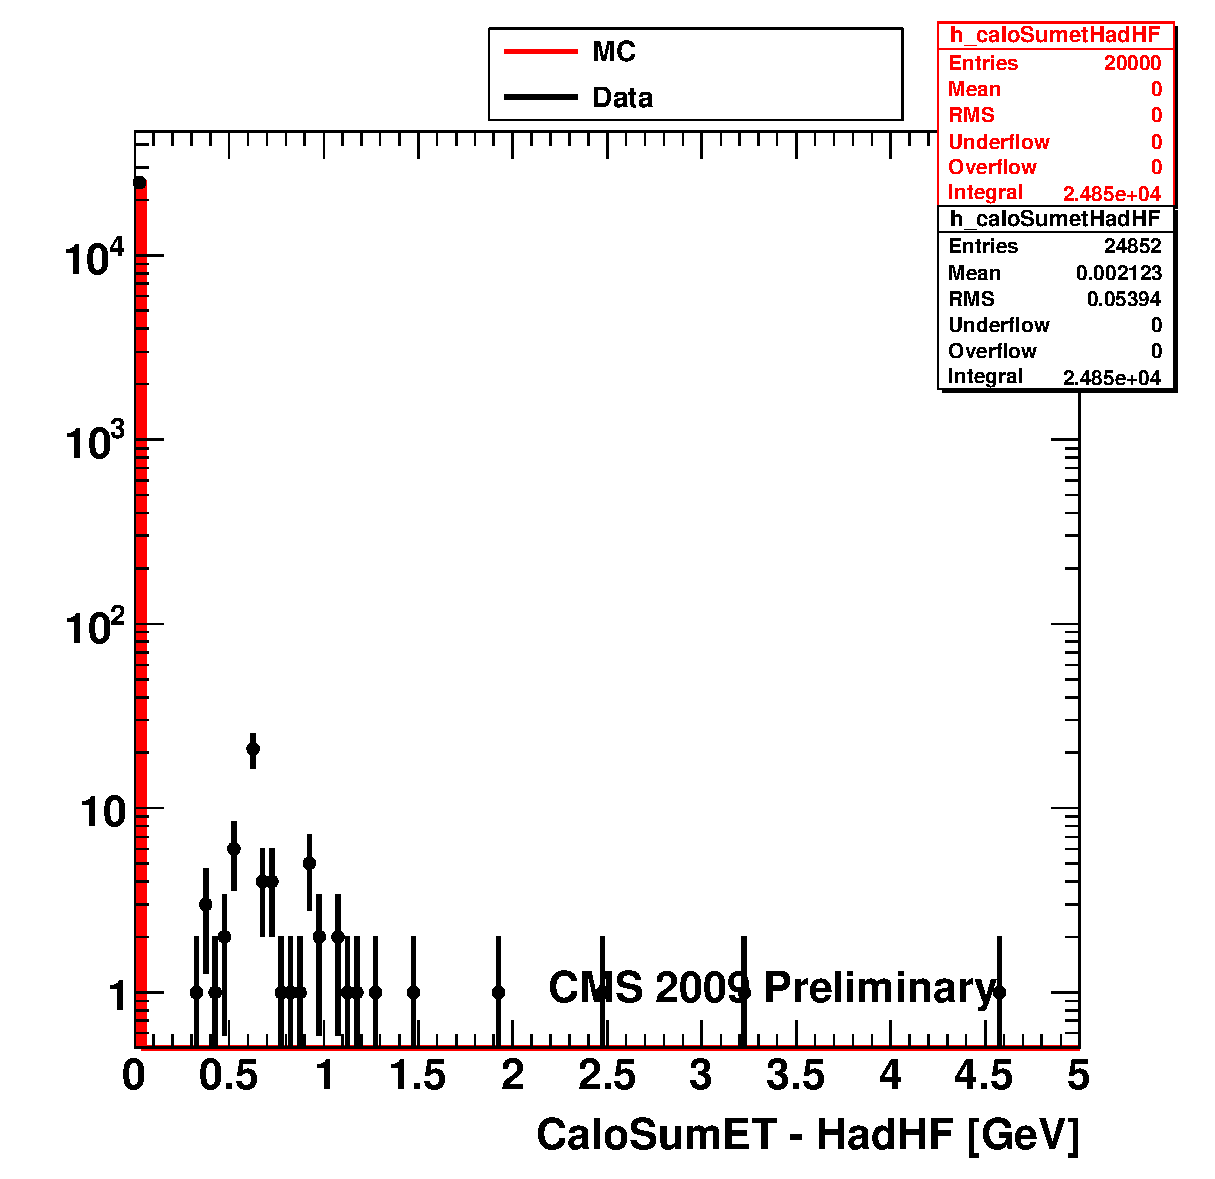
\includegraphics[width=0.33\textwidth]{plots_CaloNoise/h_caloSumetHadHF.eps} \\
 \end{tabular}
 \caption{\small $\sumet$ distributions in noise-only (red-filled area) and selected ZeroBias data (black dots) from
run 124022 in different calorimeter sub-detectors. In the HF plots, entries outside the first bin correspond to the PMT
window hits.\label{fig:subdet_CaloSumET}}
\end{figure}

\begin{figure}[h!]
 \centering
 \begin{tabular}{ll}
  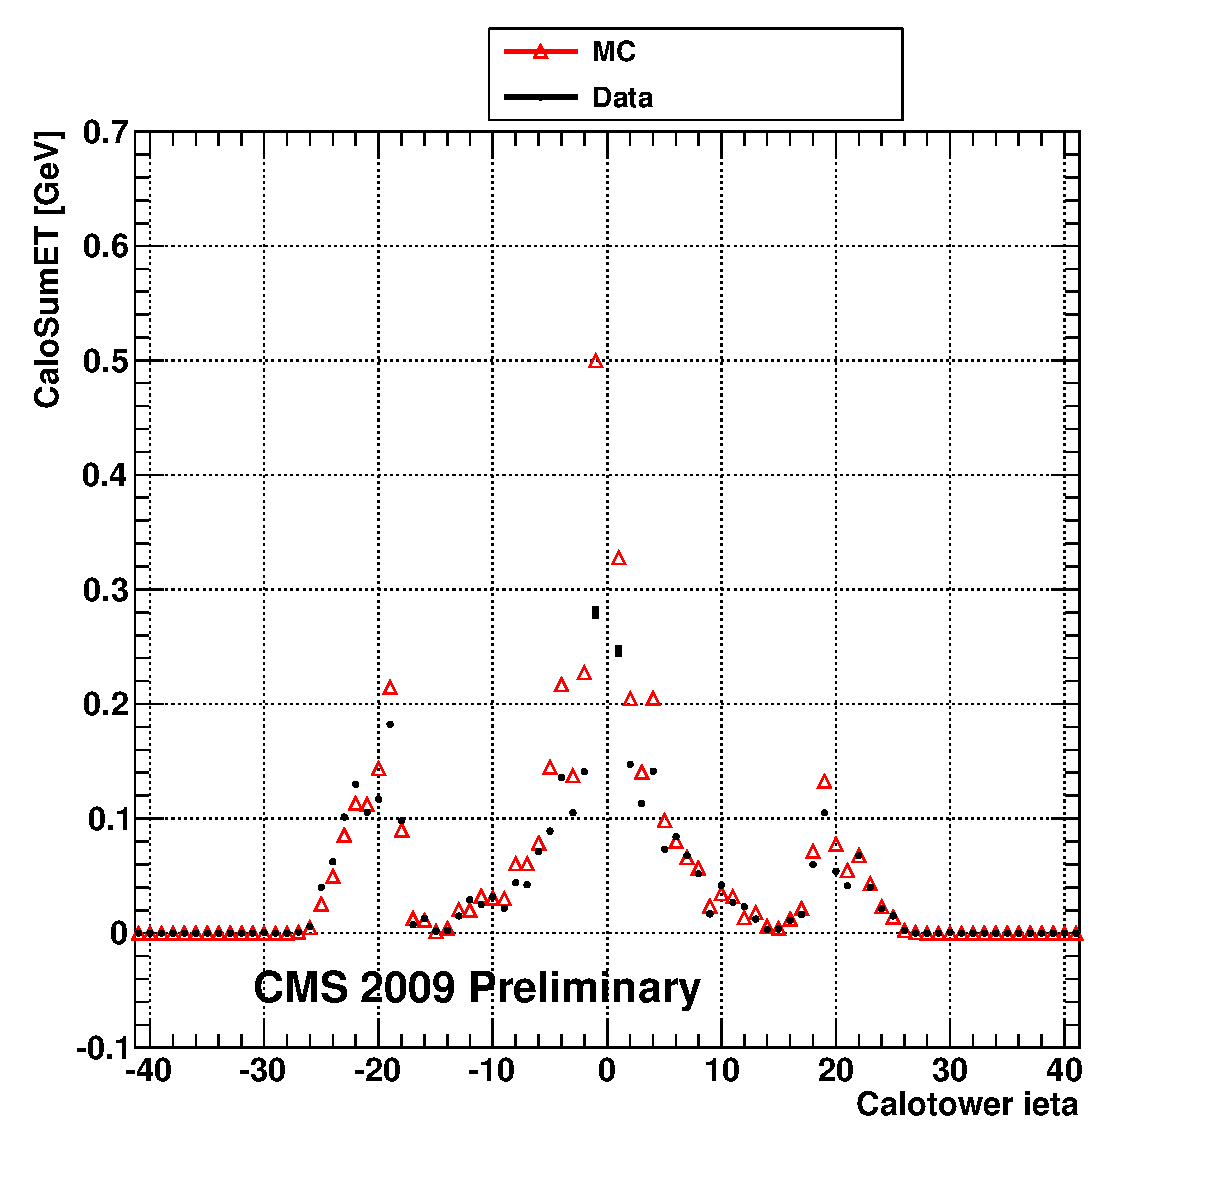
\includegraphics[width=0.33\textwidth]{plots_CaloNoise/g_caloSumetMean_vs_ieta_ZB.eps} &
  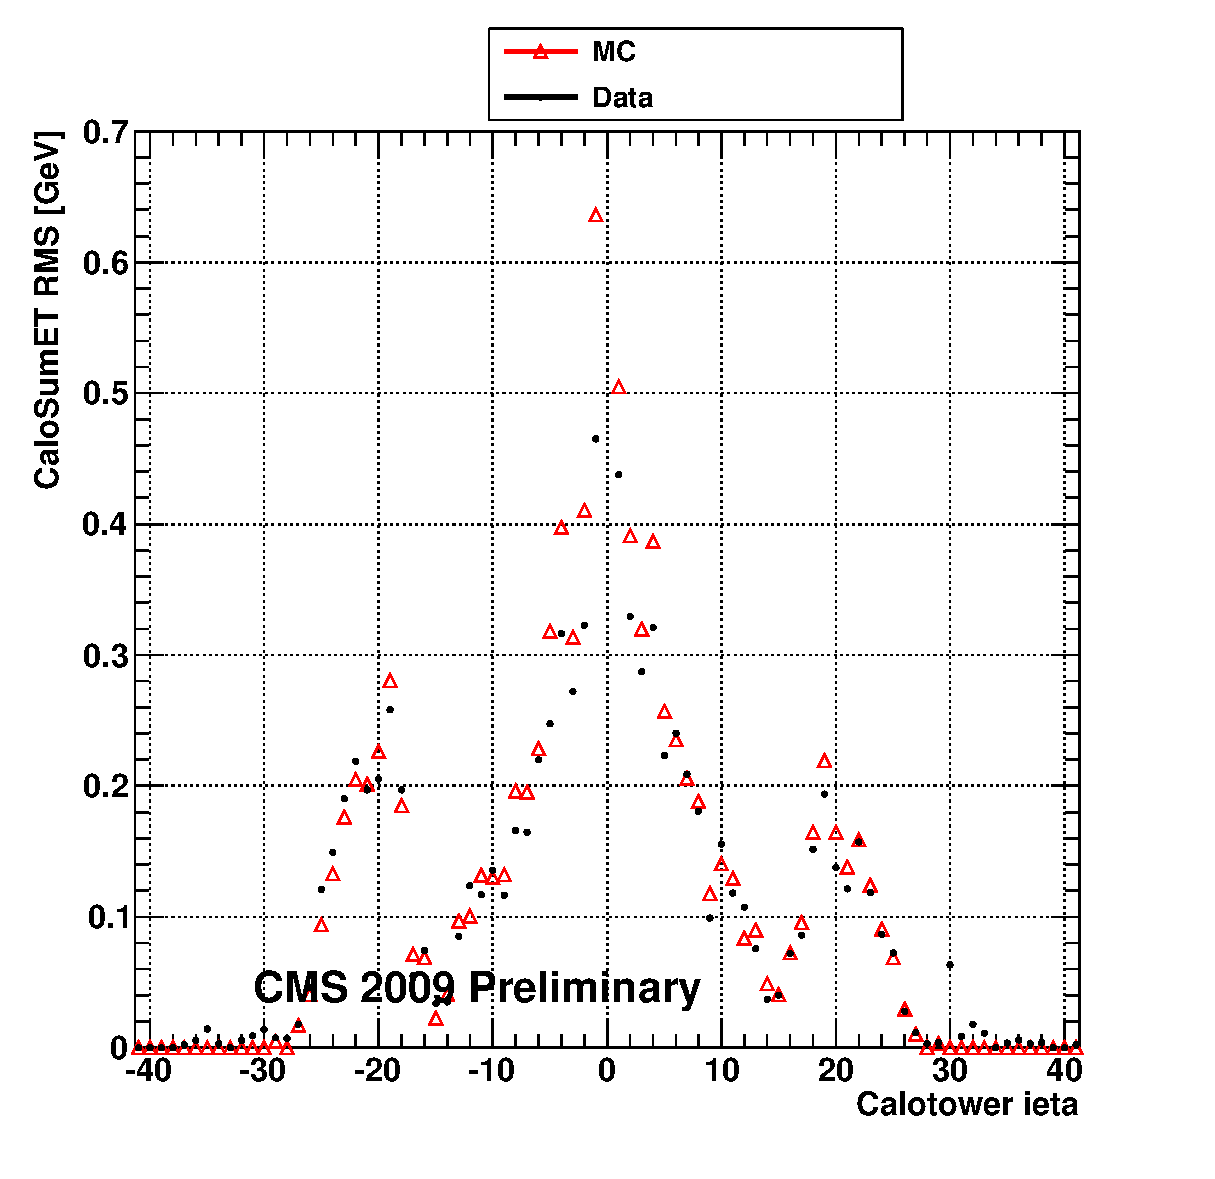
\includegraphics[width=0.33\textwidth]{plots_CaloNoise/g_caloSumetRMS_vs_ieta_ZB.eps} \\
 \end{tabular}
 \caption{\small Comparison of the $\sumet$ Mean and RMS vs. calotower $i\eta$ index between noise-only
          Monte Carlo and selected ZeroBias data.\label{fig:SumET_MeanRMS_vs_ieta_ZB}}
\end{figure}

\clearpage
